% !TeX root = ../dokumentation.tex

\chapter{Technische Umsetzung}


\section{Architektur}

\subsection{Übersicht der Services}
Hier steht Text. Hier steht Text. Hier steht Text. Hier steht Text.

\begin{figure}[!htbp]
    \centering    
    \usetikzlibrary{positioning}
    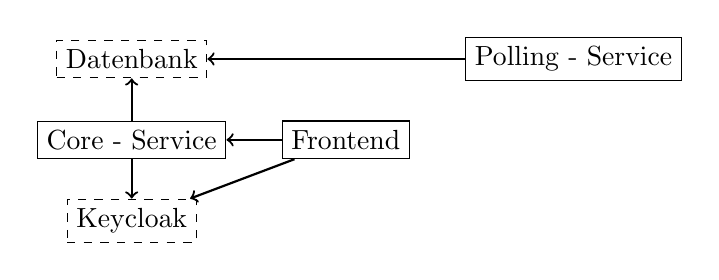
\begin{tikzpicture}
        \matrix [column sep=7mm, row sep=5mm] {
            \node (database) [draw, shape=rectangle, dashed] {Datenbank}; &&
            \node (polling_service) [draw, shape=rectangle] {Polling - Service}; \\
            \node (core_service) [draw, shape=rectangle] {Core - Service}; &
            \node (frontend) [draw, shape=rectangle] {Frontend}; \\
            \node (keycloak) [draw, shape=rectangle, dashed] {Keycloak}; \\
            };
            \draw[->, thick] (core_service) -- (database);
            \draw[->, thick] (frontend) -- (core_service);
            \draw[->, thick] (polling_service) -- (database);
            \draw[->, thick] (core_service) -- (keycloak);
            \draw[->, thick] (frontend) -- (keycloak);
        \end{tikzpicture}        
\caption{Diagramm – Darstellung der Service Architektur}
\end{figure}

\subsection{CI/CD Infrastrukture}
\subsubsection{Übersicht der Standard CI-Pipline}
Hier steht Text. Hier steht Text. Hier steht Text. Hier steht Text.

\begin{figure}[!htbp]
    \centering    
    \usetikzlibrary{positioning}
    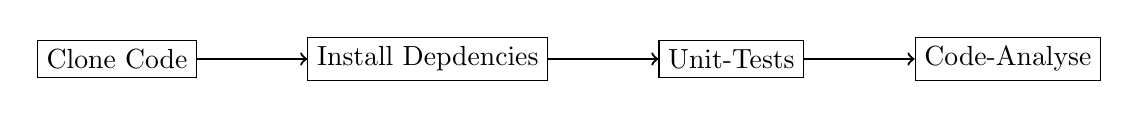
\begin{tikzpicture}
        \matrix [column sep=7mm, row sep=5mm] {
            \node (clone) [draw, shape=rectangle] {Clone Code}; &&
            \node (npm_setup) [draw, shape=rectangle] {Install Depdencies}; &&
            \node (unit_test) [draw, shape=rectangle] {Unit-Tests}; &&
            \node (sonar) [draw, shape=rectangle] {Code-Analyse}; \\
            };
            \draw[->, thick] (clone) -- (npm_setup);
            \draw[->, thick] (npm_setup) -- (unit_test);
            \draw[->, thick] (unit_test) -- (sonar);
        \end{tikzpicture}        
\caption{Diagramm – Darstellung der Standard CI-Pipeline}
\end{figure}

\subsubsection{Übersicht der Pull-Request CI-Pipline}
Hier steht Text. Hier steht Text. Hier steht Text. Hier steht Text.

\begin{figure}[!htbp]
    \centering    
    \usetikzlibrary{positioning}
    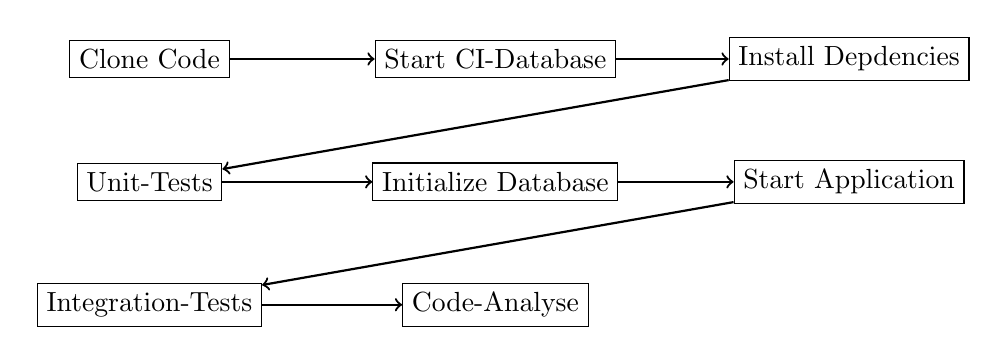
\begin{tikzpicture}
        \matrix [column sep=7mm, row sep=10mm] {
            \node (clone) [draw, shape=rectangle] {Clone Code}; &&
            \node (database) [draw, shape=rectangle] {Start CI-Database}; &&
            \node (npm_setup) [draw, shape=rectangle] {Install Depdencies}; \\
            \node (unit_test) [draw, shape=rectangle] {Unit-Tests}; &&
            \node (init_db) [draw, shape=rectangle] {Initialize Database}; &&
            \node (start_app) [draw, shape=rectangle] {Start Application}; \\
            \node (int_test) [draw, shape=rectangle] {Integration-Tests}; &&
            \node (sonar) [draw, shape=rectangle] {Code-Analyse}; \\
            };
            \draw[->, thick] (clone) -- (database);
            \draw[->, thick] (database) -- (npm_setup);
            \draw[->, thick] (npm_setup) -- (unit_test);
            \draw[->, thick] (unit_test) -- (init_db);
            \draw[->, thick] (init_db) -- (start_app);
            \draw[->, thick] (start_app) -- (int_test);
            \draw[->, thick] (int_test) -- (sonar);
        \end{tikzpicture}
\caption{Diagramm – Darstellung der Pull-Request CI-Pipeline}
\end{figure}

\subsubsection{Übersicht der Master CI-Pipline}
Hier steht Text. Hier steht Text. Hier steht Text. Hier steht Text.

\begin{figure}[!htbp]
    \centering    
    \usetikzlibrary{positioning}
    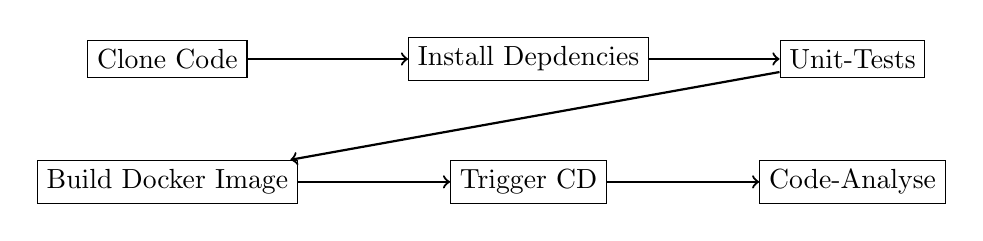
\begin{tikzpicture}
        \matrix [column sep=7mm, row sep=10mm] {
            \node (clone) [draw, shape=rectangle] {Clone Code}; &&
            \node (npm_setup) [draw, shape=rectangle] {Install Depdencies}; &&
            \node (unit_test) [draw, shape=rectangle] {Unit-Tests}; \\
            \node (docker_build) [draw, shape=rectangle] {Build Docker Image}; &&
            \node (trigger_cd) [draw, shape=rectangle] {Trigger CD}; &&
            \node (sonar) [draw, shape=rectangle] {Code-Analyse}; \\
            };
            \draw[->, thick] (clone) -- (npm_setup);
            \draw[->, thick] (npm_setup) -- (unit_test);
            \draw[->, thick] (unit_test) -- (docker_build);
            \draw[->, thick] (docker_build) -- (trigger_cd);
            \draw[->, thick] (trigger_cd) -- (sonar);
        \end{tikzpicture}
\caption{Diagramm – Darstellung der Master CI-Pipeline}
\end{figure}
\
section{Mockups}

\section{Technische Änderungen zur anfänglichen Struktur}